
\subsubsection{11.10.14}

\begin{enumerate}
	\item Время начала и окончания собрания:
	16:40 - 21:40
	\item Цели собрания:
	\begin{enumerate}
	  \item Просверлить отверстия в креплениях для балок в подъемнике.
	  
	  \item Полностью собрать направляющие подъемника с новыми креплениями.
	  
	  \item По возможности установить направляющие на робота.
	  
    \end{enumerate}
	\item Проделанная работа:
	\begin{enumerate}
	  \item Все крепления были закончены и установлены на направляющие.
      
      \item  При установке креплений для балок на направляющие выяснилось, что алюминиевый профиль тоньше, чем деталь из TETRIX-а, использовавшаяся в качестве прослойки между мебельными рейками, и из-за этого винты, которыми скреплялись направляющие, дальше выходили из отверстий и мешали мебельным рейкам раздвигаться. Было принято решение несколько сточить винты. Поскольку стачивание винта со стороны резьбы могло помешать нормальному ходу гайки по резьбе, была сточена часть шляпки, под которую затем было подложено две гайки. После этого раздвиганию направляющих ничего не мешало.
      
      \begin{figure}[H]
      	\begin{minipage}[h]{0.47\linewidth}
      		\center{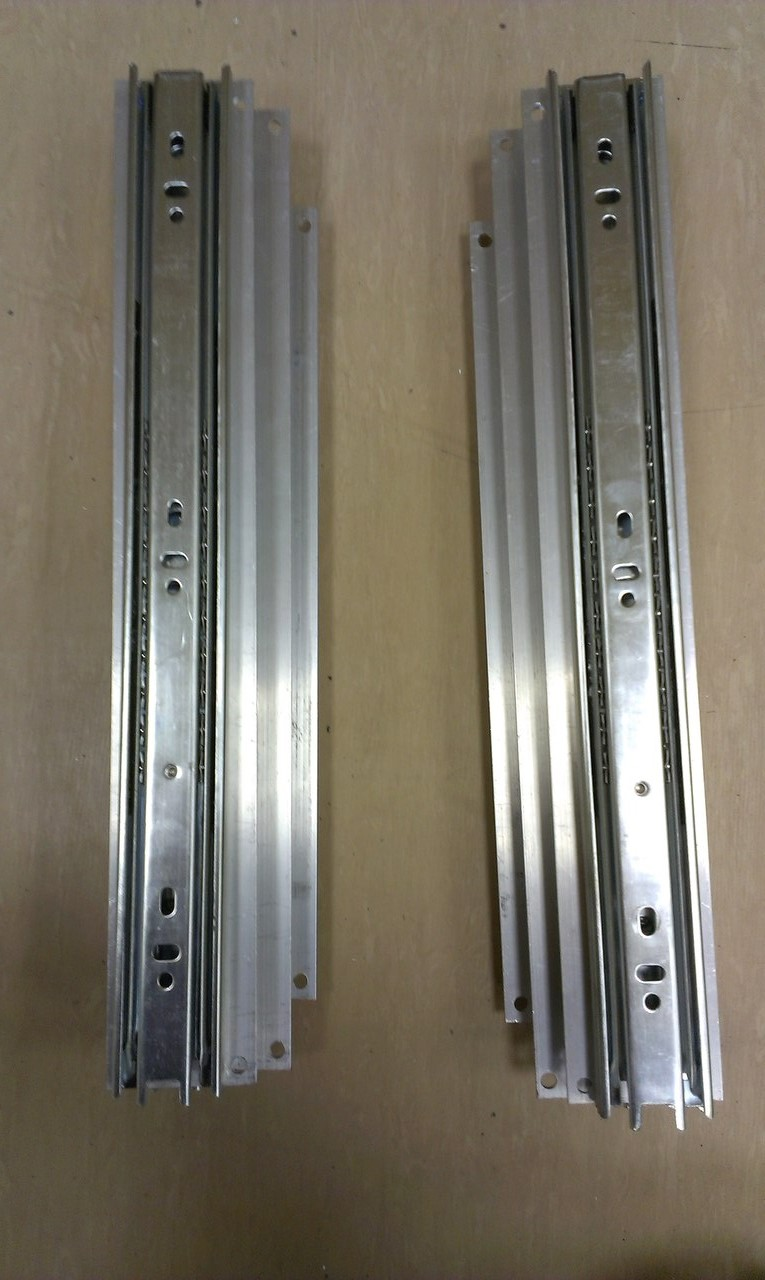
\includegraphics[scale=0.2]{days/images/7286_10gjwM}}
      	\end{minipage}
      	\begin{minipage}[h]{0.47\linewidth}
      		\center{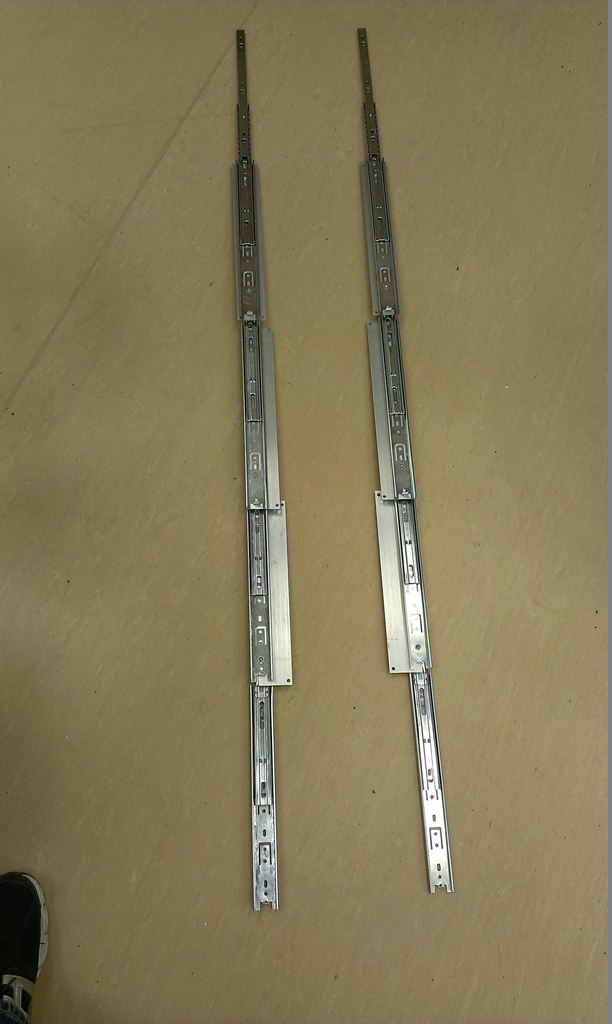
\includegraphics[scale=0.3]{days/images/tQnDFObD18I}}
      	\end{minipage}
      	\caption{Направляющие с креплениями для перекладин}
      \end{figure}
      
    \end{enumerate}
    
	\item Итоги собрания: 
	\begin{enumerate}
	  \item Направляющие собраны, но не установлены на робота.

    \end{enumerate}
    
	\item Задачи для последующих собраний:
	\begin{enumerate}
	  \item Установить направляющие на робота, собрать полноценный подъемник и испытать его в действии.
	  
    \end{enumerate}     
\end{enumerate}

\fillpage
